\chapter{A:绅士俱乐部过程改进} % Introduction chapter suppressed from the table of contents

\hypertarget{ux7ec5ux58ebux4ff1ux4e50ux90e8ux8fc7ux7a0bux6539ux8fdb}{%
\subsection{绅士俱乐部过程改进}\label{ux7ec5ux58ebux4ff1ux4e50ux90e8ux8fc7ux7a0bux6539ux8fdb}}

美国学者Dr Wheeler到日本做培训,晚上好客的日本人请他去绅士俱乐部(Esquire)。他发现年轻的女服务员腰上都有一个英文Q字牌子,便好奇地问原因。原来这家俱乐部刚完成几个月的过程改进,得到政府奖励金,所以都挂上这个Q牌(Q代表Quality质量)。

%\href{文件:ps微信截图_20230707101212.png}{350px}

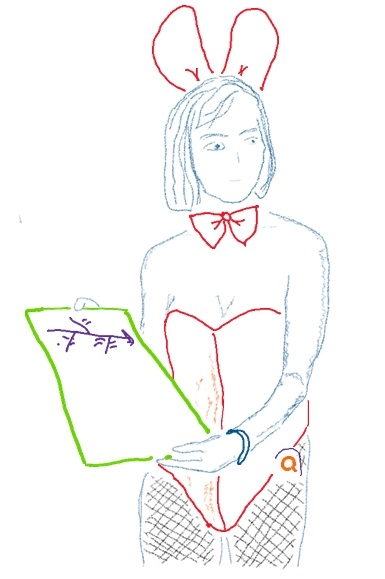
\includegraphics[width=6cm]{Esquire2Screenshot2023-10-271322091.jpg}

以下让我们看看这家俱乐部如何做过程改进。

\hypertarget{esquire-qcux5708}{%
\subsubsection{Esquire QC圈}\label{esquire-qcux5708}}

QC圈成立于1984年12月,由Sakae领导,下面的女服务员。

当时,Sakae
43岁,有七个月的经验。除了她,圈内7女服务员的年龄从19岁到23岁不等。

\hypertarget{ux7528ux4e8cux516bux539fux5219-paretoux56fe-ux8bc6ux522bux4e3bux8981ux6e90ux5934}{%
\subsubsection{用二八原则 (Pareto图)
识别主要源头}\label{ux7528ux4e8cux516bux539fux5219-paretoux56fe-ux8bc6ux522bux4e3bux8981ux6e90ux5934}}

\begin{itemize}
\tightlist
\item
  清酒 (Sake) 与 啤酒 (Beer) 是最大的源头。
\end{itemize}

%\href{文件:club55.png}{600px}

\includegraphics[width=6cm]{club55.png}

%\href{文件:club6.1.jpg}{600px}

\includegraphics[width=6cm]{club61.jpg}

每月啤酒损失量

%\href{文件:club7.1.jpg}{600px}

\includegraphics[width=6cm]{club71.jpg}

每月清酒损失量

%\href{文件:club7.2.jpg}{600px}

\includegraphics[width=6cm]{club72.jpg}

结算出平均每瓶啤酒232日元,每公升清酒1,653日元

%\href{文件:club8.1.jpg}{600px}

\includegraphics[width=6cm]{club81.jpg}

啤酒和清酒每月总损失(日元)

%\href{文件:club9.1.jpg}{600px}

\includegraphics[width=6cm]{club91.jpg}

从10月份到 2月份,啤酒和清酒的平均每月损失约 49,000 日元。

\hypertarget{ux5efaux7acbux76eeux6807}{%
\subsubsection{建立目标}\label{ux5efaux7acbux76eeux6807}}

目标:把损失减半 (少50\%):
从目前每月平均损失89瓶啤酒和17升清酒,降到(不超过)44瓶啤酒和8升清酒。

\hypertarget{ux6839ux56e0ux5206ux6790-root-cause-analysis-ux9c7cux9aa8ux56feux5206ux6790}{%
\subsubsection{根因分析 Root Cause analysis ( 鱼骨图分析
)}\label{ux6839ux56e0ux5206ux6790-root-cause-analysis-ux9c7cux9aa8ux56feux5206ux6790}}

\begin{itemize}
\tightlist
\item
  大家头脑风暴,讨论分析啤酒和清酒损失的主要原因。
\item
  根据服务员、工作流程、其他等三个主线分析。
\end{itemize}

这三组构成因果图的三个主要分支。

%\href{文件:club111.png}{600px}

\includegraphics[width=6cm]{club111.png}

\textbf{鱼骨图每个分支的主要内容如下:}

%\href{文件:club12.1.jpg}{600px}

\includegraphics[width=6cm]{club1211.jpg}

%\href{文件:club13.1.jpg}{600px}

\includegraphics[width=6cm]{club1311.jpg}

%\href{文件:club14.1.jpg}{600px}

\includegraphics[width=6cm]{club1412.jpg}

%\href{文件:club15.1.jpg}{600px}

\includegraphics[width=6cm]{club1511.jpg}

基于上面的鱼骨图分析,大家讨论并想到了以下主要理由/原因:

\begin{itemize}
\tightlist
\item
  有具体的固定位置放置账单。
\end{itemize}

\begin{itemize}
\tightlist
\item
  依赖别人。
\end{itemize}

\begin{itemize}
\tightlist
\item
  处理热清酒器不当。
\end{itemize}

\begin{itemize}
\tightlist
\item
  价格计算有误。
\end{itemize}

\begin{itemize}
\tightlist
\item
  分工有误 / 没有分配好工作。
\end{itemize}

\begin{itemize}
\tightlist
\item
  准备不足。
\end{itemize}

\begin{itemize}
\tightlist
\item
  对客户桌结算(喝了多少并收拾空酒瓶)频率不足。
\end{itemize}

\framebox{%
\begin{minipage}[t]{0.97\columnwidth}\raggedright
注意:
以上每一项都是问题的根本原因,很多人误以为针对问题本身,找改正措施便算根因分析。``5
Why'' 方法可以帮助正确找到根因,详见附件``5 Why'' 例子。
\strut
\end{minipage}}

\hypertarget{ux6539ux8fdbux63aaux65bd}{%
\subsubsection{改进措施}\label{ux6539ux8fdbux63aaux65bd}}

\begin{itemize}
\tightlist
\item
  要确保留票据在桌子上,不带走(在繁忙时段,在纸上标记消费了多少矿泉水、啤酒和日本清酒,贴在总单的后面,利于计算总账)。
\end{itemize}



\begin{itemize}
\tightlist
\item
  制定规程来分配各个区域的工作。每个小时每个区域负责人必须检查一次所有范围内的票据。
\end{itemize}

\begin{itemize}
\tightlist
\item
  送热毛巾的那位服务员负责记录新加入的客人
\end{itemize}

\begin{itemize}
\tightlist
\item
  谁接单谁负责记账,如果她要求其他人来协助记录,必须确保沟通好,检查是否已经做好记录。
\end{itemize}

\begin{itemize}
\tightlist
\item
  管理者必须对新成员提供培训,如新员工小组学习。
\end{itemize}

\begin{itemize}
\tightlist
\item
  以区域分桌,使大家清楚谁负责哪桌。
\end{itemize}

\hypertarget{ux6539ux8fdbux6548ux679c}{%
\subsubsection{改进效果}\label{ux6539ux8fdbux6548ux679c}}

\href{文件:club19.1.jpg}{600px}

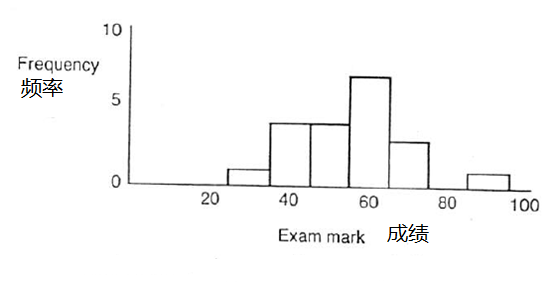
\includegraphics[width=6cm]{MA_FA1_10.png}

改进后啤酒损失降低到平均每月20瓶

%\href{文件:club20.1.jpg}{600px}

\includegraphics[width=6cm]{club201.jpg}

改进后清酒损失降低到平均每月0.6公升

%\href{文件:club20.2.jpg}{600px}

\includegraphics[width=6cm]{club202.jpg}

结算出平均每瓶啤酒232日元,每公升清酒1,653日元

%\href{文件:club21.1.jpg}{600px}

\includegraphics[width=6cm]{club211.jpg}

%\href{文件:club22.1.jpg}{600px}

\includegraphics[width=6cm]{club221.jpg}

以日元计算,啤酒和清酒的损失从每月平均49,000日元减少到5687日元,减少了43,401日元,即88\%。这一降幅远超过最初设定的50\%的目标。

\hypertarget{a3ux62a5ux544a}{%
\subsubsection{A3报告}\label{a3ux62a5ux544a}}

很多给管理层的报告都非常厚,信息太多导致管理者难以消化,所以丰田要求所有管理报告都必须精简到一张A3纸。
照片中服务员手上的就是A3报告 -\/-\/-
包含了根因分析的重点。例如你可以看见其中有鱼骨图。

\hypertarget{ux9644ux4ef6}{%
\section{参考 References}\label{ux9644ux4ef6}}

1. Wheeler, Donald J. : SPC at the Esquire Club (SPC Press 1992)

